%===============================================================================
% LaTeX sjabloon voor de bachelorproef toegepaste informatica aan HOGENT
% Meer info op https://github.com/HoGentTIN/latex-hogent-report
%===============================================================================

\documentclass[dutch,dit,thesis]{hogentreport}

% TODO:
% - If necessary, replace the option `dit`' with your own department!
%   Valid entries are dbo, dbt, dgz, dit, dlo, dog, dsa, soa
% - If you write your thesis in English (remark: only possible after getting
%   explicit approval!), remove the option "dutch," or replace with "english".

\usepackage{lipsum} % For blind text, can be removed after adding actual content

%% Pictures to include in the text can be put in the graphics/ folder
\graphicspath{{../graphics/}}

%% For source code highlighting, requires pygments to be installed
%% Compile with the -shell-escape flag!
%% \usepackage[chapter]{minted}
%% If you compile with the make_thesis.{bat,sh} script, use the following
%% import instead:
\usepackage[chapter,outputdir=../output]{minted}
\usemintedstyle{solarized-light}

%% Formatting for minted environments.
\setminted{%
    autogobble,
    frame=lines,
    breaklines,
    linenos,
    tabsize=4
}

%% Ensure the list of listings is in the table of contents
\renewcommand\listoflistingscaption{%
    \IfLanguageName{dutch}{Lijst van codefragmenten}{List of listings}
}
\renewcommand\listingscaption{%
    \IfLanguageName{dutch}{Codefragment}{Listing}
}
\renewcommand*\listoflistings{%
    \cleardoublepage\phantomsection\addcontentsline{toc}{chapter}{\listoflistingscaption}%
    \listof{listing}{\listoflistingscaption}%
}

% Other packages not already included can be imported here
% //TODO MARK: fix the glossaries package
\usepackage[acronym]{glossaries}
\makeglossaries

\newacronym{cf}{CF}{Collaborative Filtering}
\newacronym{fl}{FL}{Federated Learning}
\newacronym{dp}{DP}{Differential Privacy}

%%---------- Document metadata -------------------------------------------------
% TODO: Replace this with your own information
\author{Pushwant Sagoo}
\supervisor{Mevr. Sharon Van Hove}
\cosupervisor{Dhr. Maurice Cantaert}
\title%[Optionele ondertitel]%
    {Ontwikkeling en evaluatie van een privacy behoudend Collaborative Filtering gebaseerd aanbevelingssysteem met behulp van Federated Learning en Differential Privacy} 
\academicyear{\advance\year by -1 \the\year--\advance\year by 1 \the\year}
\examperiod{2}
\degreesought{\IfLanguageName{dutch}{Professionele bachelor in de toegepaste informatica}{Bachelor of applied computer science}}
\partialthesis{false} %% To display 'in partial fulfilment'
%\institution{Internshipcompany BVBA.}

%% Add global exceptions to the hyphenation here
\hyphenation{back-slash}

%% The bibliography (style and settings are  found in hogentthesis.cls)
\addbibresource{bachproef.bib}            %% Bibliography file
\addbibresource{../voorstel/voorstel.bib} %% Bibliography research proposal
\defbibheading{bibempty}{}

%% Prevent empty pages for right-handed chapter starts in twoside mode
\renewcommand{\cleardoublepage}{\clearpage}

\renewcommand{\arraystretch}{1.2}

%% Content starts here.
\begin{document}

%---------- Front matter -------------------------------------------------------

\frontmatter

\hypersetup{pageanchor=false} %% Disable page numbering references
%% Render a Dutch outer title page if the main language is English
\IfLanguageName{english}{%
    %% If necessary, information can be changed here
    \degreesought{Professionele Bachelor toegepaste informatica}%
    \begin{otherlanguage}{dutch}%
       \maketitle%
    \end{otherlanguage}%
}{}

%% Generates title page content
\maketitle
\hypersetup{pageanchor=true}

\input{voorwoord}
%%=============================================================================
%% Samenvatting
%%=============================================================================

% TODO: De "abstract" of samenvatting is een kernachtige (~ 1 blz. voor een
% thesis) synthese van het document.
%
% Een goede abstract biedt een kernachtig antwoord op volgende vragen:
%
% 1. Waarover gaat de bachelorproef?
% 2. Waarom heb je er over geschreven?
% 3. Hoe heb je het onderzoek uitgevoerd?
% 4. Wat waren de resultaten? Wat blijkt uit je onderzoek?
% 5. Wat betekenen je resultaten? Wat is de relevantie voor het werkveld?
%
% Daarom bestaat een abstract uit volgende componenten:
%
% - inleiding + kaderen thema
% - probleemstelling
% - (centrale) onderzoeksvraag
% - onderzoeksdoelstelling
% - methodologie
% - resultaten (beperk tot de belangrijkste, relevant voor de onderzoeksvraag)
% - conclusies, aanbevelingen, beperkingen
%
% LET OP! Een samenvatting is GEEN voorwoord!

%%---------- Nederlandse samenvatting -----------------------------------------
%
% TODO: Als je je bachelorproef in het Engels schrijft, moet je eerst een
% Nederlandse samenvatting invoegen. Haal daarvoor onderstaande code uit
% commentaar.
% Wie zijn bachelorproef in het Nederlands schrijft, kan dit negeren, de inhoud
% wordt niet in het document ingevoegd.

\IfLanguageName{english}{%
\selectlanguage{dutch}
\chapter*{Samenvatting}
\lipsum[1-4]
\selectlanguage{english}
}{}

%%---------- Samenvatting -----------------------------------------------------
% De samenvatting in de hoofdtaal van het document

\chapter*{\IfLanguageName{dutch}{Samenvatting}{Abstract}}
Dit onderzoek richt zich op het ontwerpen en ontwikkelen van een privacy behoudend Collaborative Filtering (CF) aanbevelingssysteem, waarbij Federated Learning (FL) en Differential Privacy (DP) worden geïntegreerd om gepersonaliseerde aanbevelingen te leveren zonder de privacy van gebruikers in gevaar te brengen. In tegenstelling tot traditionele CF-systemen, die afhankelijk zijn van gecentraliseerde datasets, worden in dit systeem gebruikersdata lokaal op hun eigen apparaten bewaard. Via FL worden alleen geaggregeerde modelupdates, verrijkt met zorgvuldig berekende ruis door middel van DP, naar een centraal globaal model gestuurd. Deze ruis wordt toegevoegd aan de parameters die tijdens het federale leerproces worden gedeeld, waardoor de privacy van individuele gebruikers wordt gewaarborgd zonder de nauwkeurigheid van het aanbevelingssysteem significant aan te tasten.

Het doel van dit onderzoek is het ontwikkelen van een proof of concept (POC) dat aantoont hoe FL en DP effectief kunnen worden gecombineerd om een privacy-behoudend CF-systeem te creëren. Hierbij ligt de focus op het vinden van een optimale balans tussen de kwaliteit van de aanbevelingen en het niveau van gegevensbescherming. Verwacht wordt dat deze aanpak de privacyrisico's van traditionele aanbevelingssystemen aanzienlijk vermindert, terwijl de relevantie en precisie van de aanbevelingen behouden blijven.

Dit onderzoek draagt bij aan een innovatieve oplossing die toepasbaar is in diverse sectoren waar gepersonaliseerde aanbevelingen worden ingezet. Bovendien heeft deze aanpak het potentieel om het vertrouwen van gebruikers te vergroten en de bedrijfswaarde te verhogen door een transparante en veilige verwerking van gevoelige data.


%---------- Inhoud, lijst figuren, ... -----------------------------------------

\tableofcontents

% In a list of figures, the complete caption will be included. To prevent this,
% ALWAYS add a short description in the caption!
%
%  \caption[short description]{elaborate description}
%
% If you do, only the short description will be used in the list of figures

\listoffigures

% If you included tables and/or source code listings, uncomment the appropriate
% lines.
\listoftables

\listoflistings

% Als je een lijst van afkortingen of termen wil toevoegen, dan hoort die
% hier thuis. Gebruik bijvoorbeeld de ``glossaries'' package.
% https://www.overleaf.com/learn/latex/Glossaries
\printglossary[type=\acronymtype, title="Lijst van afkortingen", toctitle="Lijst van afkortingen"]

%---------- Kern ---------------------------------------------------------------

\mainmatter{}

% De eerste hoofdstukken van een bachelorproef zijn meestal een inleiding op
% het onderwerp, literatuurstudie en verantwoording methodologie.
% Aarzel niet om een meer beschrijvende titel aan deze hoofdstukken te geven of
% om bijvoorbeeld de inleiding en/of stand van zaken over meerdere hoofdstukken
% te verspreiden!

%%=============================================================================
%% Inleiding
%%=============================================================================

\chapter{\IfLanguageName{dutch}{Inleiding}{Introduction}}%
\label{ch:inleiding}

% De inleiding moet de lezer net genoeg informatie verschaffen om het onderwerp te begrijpen en in te zien waarom de onderzoeksvraag de moeite waard is om te onderzoeken. In de inleiding ga je literatuurverwijzingen beperken, zodat de tekst vlot leesbaar blijft. Je kan de inleiding verder onderverdelen in secties als dit de tekst verduidelijkt. Zaken die aan bod kunnen komen in de inleiding~\autocite{Pollefliet2011}:

% \begin{itemize}
%   \item context, achtergrond
%   \item afbakenen van het onderwerp
%   \item verantwoording van het onderwerp, methodologie
%   \item probleemstelling
%   \item onderzoeksdoelstelling
%   \item onderzoeksvraag
%   \item \ldots
% \end{itemize}

Aanbevelingssystemen zijn geavanceerde tools die gebruikmaken van grote hoeveelheden data om gepersonaliseerde suggesties te doen aan gebruikers. Deze systemen spelen een cruciale rol in diverse sectoren, zoals e-commerce, streamingdiensten, sociale media en entertainment. Ze helpen gebruikers bij het ontdekken van relevante producten, diensten of content, zoals het aanraden van films op een streamingplatform of het tonen van gerichte advertenties om klanten te verleiden tot aankopen. Door gebruik te maken van gebruikersgedrag, voorkeuren en interactiepatronen, kunnen deze systemen een gepersonaliseerde ervaring bieden die zowel de gebruikers tevreden stelt als de bedrijfsdoelen ondersteunt.

Dit onderzoek richt zich specifiek op aanbevelingssystemen binnen de entertainmentsector, met een focus op films. Hierbij worden filmgerelateerde data en gebruikersvoorkeuren gebruikt voor de ontwikkeling en evaluatie van het systeem. Het doel is om een systeem te creëren dat niet alleen nauwkeurige en relevante aanbevelingen doet, maar ook de privacy van gebruikers respecteert en beschermt.

\section{\IfLanguageName{dutch}{Probleemstelling}{Problem Statement}}%
\label{sec:probleemstelling}

% Uit je probleemstelling moet duidelijk zijn dat je onderzoek een meerwaarde heeft voor een concrete doelgroep. De doelgroep moet goed gedefinieerd en afgelijnd zijn. Doelgroepen als ``bedrijven,'' ``KMO's'', systeembeheerders, enz.~zijn nog te vaag. Als je een lijstje kan maken van de personen/organisaties die een meerwaarde zullen vinden in deze bachelorproef (dit is eigenlijk je steekproefkader), dan is dat een indicatie dat de doelgroep goed gedefinieerd is. Dit kan een enkel bedrijf zijn of zelfs één persoon (je co-promotor/opdrachtgever).

Een veelgehoorde aanname in de wereld van aanbevelingssystemen is dat hoe meer data een systeem kan verwerken, hoe nauwkeuriger en relevanter de aanbevelingen worden. Traditionele aanbevelingssystemen maken vaak gebruik van methoden zoals Collaborative Filtering (CF) en Content-Based Recommendations (CB). CF richt zich op het identificeren van patronen in gebruikersgedrag, terwijl CB aanbevelingen doet op basis van de eigenschappen van items, zoals genre of beschrijvingen. Daarnaast zijn er moderne methoden die gebruikmaken van geavanceerde technieken zoals neurale netwerken en deep learning.

Echter, deze systemen zijn vaak afhankelijk van gecentraliseerde datasets, wat ernstige privacyrisico's met zich meebrengt. Gebruikersdata wordt meestal opgeslagen en verwerkt op centrale servers, wat het risico op datalekken en misbruik vergroot. Bovendien kunnen gebruikers zich zorgen maken over hoe hun persoonlijke gegevens worden gebruikt, wat het vertrouwen in dergelijke systemen kan ondermijnen. 

\section{\IfLanguageName{dutch}{Onderzoeksvraag}{Research question}}%
\label{sec:onderzoeksvraag}

% Wees zo concreet mogelijk bij het formuleren van je onderzoeksvraag. Een onderzoeksvraag is trouwens iets waar nog niemand op dit moment een antwoord heeft (voor zover je kan nagaan). Het opzoeken van bestaande informatie (bv. ``welke tools bestaan er voor deze toepassing?'') is dus geen onderzoeksvraag. Je kan de onderzoeksvraag verder specifiëren in deelvragen. Bv.~als je onderzoek gaat over performantiemetingen, dan 

Dit roept de vraag op: \textit{Hoe kunnen we een aanbevelingssysteem ontwikkelen dat nauwkeurige en gepersonaliseerde aanbevelingen doet zonder de privacy van gebruikers in gevaar te brengen?}

Deze hoofdvraag kan worden opgesplitst in de volgende deelvragen:
\begin{itemize}
  \item \textbf{Hoe kan Federated Learning worden toegepast om een Collaborative Filtering-systeem te ontwikkelen waarbij gebruikersdata lokaal blijft?}
  Federated Learning maakt het mogelijk om machine learning-modellen te trainen zonder dat gebruikersdata wordt gedeeld of opgeslagen op een centrale server. In plaats daarvan wordt het model getraind op het apparaat van de gebruiker, en alleen geaggregeerde updates worden naar een globaal model gestuurd. Dit minimaliseert het risico op datalekken en beschermt de privacy van gebruikers.
  \item \textbf{Hoe kan Differential Privacy worden geïntegreerd om berekende ruis toe te voegen aan de parameters die naar het globale model worden gestuurd?}
  Differential Privacy voegt gecontroleerde ruis toe aan de data of modelparameters voordat deze worden gedeeld. Dit zorgt ervoor dat individuele gebruikers niet kunnen worden geïdentificeerd, zelfs niet wanneer de data wordt geanalyseerd.
  \item \textbf{Wat is de balans tussen de nauwkeurigheid van aanbevelingen en het niveau van gegevensbescherming?}
  Het toevoegen van ruis kan de nauwkeurigheid van het model beïnvloeden. Daarom is het belangrijk om een optimale balans te vinden tussen het beschermen van privacy en het behouden van de kwaliteit van de aanbevelingen.
\end{itemize}

\section{\IfLanguageName{dutch}{Onderzoeksdoelstelling}{Research objective}}%
\label{sec:onderzoeksdoelstelling}

% Wat is het beoogde resultaat van je bachelorproef? Wat zijn de criteria voor succes? Beschrijf die zo concreet mogelijk. Gaat het bv.\ om een proof-of-concept, een prototype, een verslag met aanbevelingen, een vergelijkende studie, enz.

Het doel van dit onderzoek is het ontwikkelen van een werkend prototype van een privacy-preserverend Collaborative Filtering-systeem dat gebruikmaakt van Federated Learning (FL) en Differential Privacy (DP). Volgende aspecten zijn van belang:
\begin{itemize}
  \item \textit{Ontwikkeling van een CF-systeem met Federated Learning}
  \\
  Het systeem moet gebruikersdata lokaal verwerken en alleen geanonimiseerde updates naar een globaal model sturen. Dit vermindert het risico op datalekken en zorgt ervoor dat gevoelige informatie nooit centraal wordt opgeslagen.
  \item \textit{Integratie van Differential Privacy}
  \\
  Door berekende ruis toe te voegen aan de parameters die naar het globale model worden gestuurd, wordt de privacy van individuele gebruikers beschermd.
  \item \textit{Evaluatie van de balans tussen nauwkeurigheid en privacy}
  \\
  Het systeem moet worden getest en geëvalueerd om de optimale balans te vinden tussen de kwaliteit van de aanbevelingen en het niveau van gegevensbescherming.
\end{itemize}

\section{\IfLanguageName{dutch}{Opzet van deze bachelorproef}{Structure of this bachelor thesis}}%
\label{sec:opzet-bachelorproef}

% Het is gebruikelijk aan het einde van de inleiding een overzicht te
% geven van de opbouw van de rest van de tekst. Deze sectie bevat al een aanzet
% die je kan aanvullen/aanpassen in functie van je eigen tekst.

De rest van deze bachelorproef is als volgt opgebouwd:

In Hoofdstuk~\ref{ch:stand-van-zaken} wordt een overzicht gegeven van de stand van zaken binnen het onderzoeksdomein, op basis van een literatuurstudie.

In Hoofdstuk~\ref{ch:methodologie} wordt de methodologie toegelicht en worden de gebruikte onderzoekstechnieken besproken om een antwoord te kunnen formuleren op de onderzoeksvragen.

% TODO: Vul hier aan voor je eigen hoofstukken, één of twee zinnen per hoofdstuk

In Hoofdstuk~\ref{ch:conclusie}, tenslotte, wordt de conclusie gegeven en een antwoord geformuleerd op de onderzoeksvragen. Daarbij wordt ook een aanzet gegeven voor toekomstig onderzoek binnen dit domein.
\chapter{\IfLanguageName{dutch}{Stand van zaken}{State of the art}}%
\label{ch:stand-van-zaken}

% Tip: Begin elk hoofdstuk met een paragraaf inleiding die beschrijft hoe
% dit hoofdstuk past binnen het geheel van de bachelorproef. Geef in het
% bijzonder aan wat de link is met het vorige en volgende hoofdstuk.

% Pas na deze inleidende paragraaf komt de eerste sectiehoofding.

\section{Inleiding tot aanbevelingssytemen}
Aanbevelingssystemen zijn algoritmes en software tools met als doel om gepersonaliseerde aanbevelingen op basis van gelijkenis van items, gebruikersprofiel of andere kenmerken, te geven aan gebruikers \autocite{Patel2020, Patel2023}. De aanbevelingen worden gemaakt aan de hand van verschillende besluitvormingsprocessen, zoals welk nieuws hij leest, naar welke film hij kijkt of naar welke muziek hij luistert \autocite{Patel2017}. De kernfunctie van een aanbevelingssysteem is het voorspellen van de relevantie of voorkeur die een gebruiker aan een item zou toekennen, waarbij de enorme hoveelheid informatie gefilterd wordt en gebruikers enkel keuzes krijgen voorgeschoteld die op hun interesses zijn afgestemd \autocite{Fkih2022}. Anders gezegd kunnen aanbevelingsystemen gezien worden als functies die informatie over de voorkeuren van een gebruiker (bijv. over films) als invoer nemen en een voorspelling doen over de beoordeling die een gebruiker zou geven aan andere gewenste items (bijv. nieuwe beschikbare films) en het uitvoer zijn aanbevelingen van deze items \autocite{Milano2020}. Aanbevelingen kunnen gaan over een breed scala aan items, waaronder producten in e-commerce, films, muziek, nieuwsartikelen en contacten op sociale media.
\subsection{Toepassingen van aanbevelingssystemen}
De toepassingen van aanbevelingssystemen zijn uitgebreid en doordringen talloze domeinen. Een van de meeste bekende toepassing is in e-commerce, waar producten aanbevelen aan klanten op basis van hun aankoopgeschiedenis en surfgedrag, zoals de Amazon "item-to-item \ac{cf}" algoritme \autocite{Patel2023, Patel2020}.
In de entertaintment industrie bij het aanbevelen van films op Netflix, IMDB of MovieLens en muziek \autocite{Patel2020, Roy2022}. Op sociale media platformen zoals Facebook en Twitter worden aanbevelingen gedaan voor nieuwe personen en pagina's \autocite{Patel2023}. Zelfs de advertenties op deze platformen vaak afgestemd op de intresses van de gebruiker \autocite{Patel2020}.
In het onderzoek \textcite{Agapito2016} wordt DIETOS (DIET Organizer System) geïntroduceerd, een webgebaseerd aanbevelingssysteem dat gepersonaliseerd voedingsadvies biedt op basis van een gezondheidsprofiel van de gebruiker. Dit profiel wordt opgebouwd via dynamische vragenlijsten die zijn ontwikkeld en gevalideerd door medische professionals. Het systeem richt zich specifiek op het aanbevelen van geschikte voedingsmiddelen voor personen met chronische aandoeningen zoals diabetes, hypertensie en chronische nierziekten. Toeristen kunnen ook geholpen worden bij het plannen van hun reis door aanbevelingen te geven over bezienswaardigheden, restaurants en hotels \autocite{Roy2022, Patel2023}.
\subsection{Wat maakt ze nuttig?}
\section{\ac{cf} gebaseerde aanbevelingssystemen}
\section{Toepassing \ac{fl} techniek}
\section{\ac{dp} framework}
\section{Evalueren van aanbevelingssystemen}

Dit hoofdstuk bevat je literatuurstudie. De inhoud gaat verder op de inleiding, maar zal het onderwerp van de bachelorproef *diepgaand* uitspitten. De bedoeling is dat de lezer na lezing van dit hoofdstuk helemaal op de hoogte is van de huidige stand van zaken (state-of-the-art) in het onderzoeksdomein. Iemand die niet vertrouwd is met het onderwerp, weet nu voldoende om de rest van het verhaal te kunnen volgen, zonder dat die er nog andere informatie moet over opzoeken \autocite{Pollefliet2011}.

Je verwijst bij elke bewering die je doet, vakterm die je introduceert, enz.\ naar je bronnen. In \LaTeX{} kan dat met het commando \texttt{$\backslash${textcite\{\}}} of \texttt{$\backslash${autocite\{\}}}. Als argument van het commando geef je de ``sleutel'' van een ``record'' in een bibliografische databank in het Bib\LaTeX{}-formaat (een tekstbestand). Als je expliciet naar de auteur verwijst in de zin (narratieve referentie), gebruik je \texttt{$\backslash${}textcite\{\}}. Soms is de auteursnaam niet expliciet een onderdeel van de zin, dan gebruik je \texttt{$\backslash${}autocite\{\}} (referentie tussen haakjes). Dit gebruik je bv.~bij een citaat, of om in het bijschrift van een overgenomen afbeelding, broncode, tabel, enz. te verwijzen naar de bron. In de volgende paragraaf een voorbeeld van elk.

\textcite{Knuth1998} schreef een van de standaardwerken over sorteer- en zoekalgoritmen. Experten zijn het erover eens dat cloud computing een interessante opportuniteit vormen, zowel voor gebruikers als voor dienstverleners op vlak van informatietechnologie~\autocite{Creeger2009}.

Let er ook op: het \texttt{cite}-commando voor de punt, dus binnen de zin. Je verwijst meteen naar een bron in de eerste zin die erop gebaseerd is, dus niet pas op het einde van een paragraaf.

\begin{figure}
  \centering
  \includegraphics[width=0.8\textwidth]{grail.jpg}
  \caption[Voorbeeld figuur.]{\label{fig:grail}Voorbeeld van invoegen van een figuur. Zorg altijd voor een uitgebreid bijschrift dat de figuur volledig beschrijft zonder in de tekst te moeten gaan zoeken. Vergeet ook je bronvermelding niet!}
\end{figure}

\begin{listing}
  \begin{minted}{python}
    import pandas as pd
    import seaborn as sns

    penguins = sns.load_dataset('penguins')
    sns.relplot(data=penguins, x="flipper_length_mm", y="bill_length_mm", hue="species")
  \end{minted}
  \caption[Voorbeeld codefragment]{Voorbeeld van het invoegen van een codefragment.}
\end{listing}

\lipsum[7-20]

\begin{table}
  \centering
  \begin{tabular}{lcr}
    \toprule
    \textbf{Kolom 1} & \textbf{Kolom 2} & \textbf{Kolom 3} \\
    $\alpha$         & $\beta$          & $\gamma$         \\
    \midrule
    A                & 10.230           & a                \\
    B                & 45.678           & b                \\
    C                & 99.987           & c                \\
    \bottomrule
  \end{tabular}
  \caption[Voorbeeld tabel]{\label{tab:example}Voorbeeld van een tabel.}
\end{table}


\input{methodologie}

% Voeg hier je eigen hoofdstukken toe die de ``corpus'' van je bachelorproef
% vormen. De structuur en titels hangen af van je eigen onderzoek. Je kan bv.
% elke fase in je onderzoek in een apart hoofdstuk bespreken.

%\input{...}
%\input{...}
%...

\input{conclusie}

%---------- Bijlagen -----------------------------------------------------------

\appendix

\chapter{Onderzoeksvoorstel}

Het onderwerp van deze bachelorproef is gebaseerd op een onderzoeksvoorstel dat vooraf werd beoordeeld door de promotor. Dat voorstel is opgenomen in deze bijlage.
% //TODO MARK: voeg uitleg over verschillen tussen voorstel en bachelorproef toe 
%% TODO: 
\section*{Samenvatting}

% Kopieer en plak hier de samenvatting (abstract) van je onderzoeksvoorstel.
Het ontwikkelen van een privacy preserverende hybride aanbevelingssysteem biedt kansen om gepersonaliseerde aanbevelingen te leveren zonder inbreuk te maken op de privacy van gebruikers, wat waardevol is voor allerlei sectoren die met gepersonaliseerde informatie werken. Dit onderzoek richt zich op het ontwikkelen van een hybride systeem dat zowel Content Based (CB) als Collaborative Filtering (CF) technieken combineert, waarbij Federated Learning (FL) en Differential Privacy (DP) methodieken worden ingezet om de anonimiteit van gebruikers te garanderen en tegelijkertijd accurate aanbevelingen te doen. Het CB deel maakt gebruik van FL, waardoor de data van gebruikers op hun eigen toestel blijft en enkel geanonimiseerde updates worden naar een centrale server gestuurd, zodat aanbevelingen op basis van persoonlijke voorkeuren lokaal kunnen worden gegenereerd zonder centrale opslag voor gevoelige informatie. Voor het CF deel, dat gebruikmaakt van grotere geaggregeerde datasets, wordt DP toegepast om de gebruikersgegevens verder te beschermen door ruis toe te voegen aan de data voordat deze wordt verwerkt, zelfs tijdens verwerken van gemeenschappelijke voorkeurspatronen. Het doel is een werkend prototype te ontwikkelen dat nauwkeurige aanbevelingen genereert, waarbij de balans tussen aanbevelingskwaliteit en gegevensbescherming wordt geëvalueerd. Verwacht wordt dat deze aanpak de privacyrisico's van traditionele systemen aanzienlijk verlaagt, terwijl de relevantie en precisie van aanbevelingen behouden blijft. Dit onderzoek draagt bij aan een waardevolle oplossing voor privacyvriendelijke, op maat gemaakte aanbevelingen aan te bieden die voldoen aan de eisen van privacywetgevingen en bovendien die een breed scala aan toepassingen hebben in verschillende sectoren. Daarnaast vergroot deze aanpak het gebruikersvertrouwen en verhoogt de klantwaarde.

% Verwijzing naar het bestand met de inhoud van het onderzoeksvoorstel
%---------- Inleiding ---------------------------------------------------------

% TODO: Is dit voorstel gebaseerd op een paper van Research Methods die je
% vorig jaar hebt ingediend? Heb je daarbij eventueel samengewerkt met een
% andere student?
% Zo ja, haal dan de tekst hieronder uit commentaar en pas aan.

%\paragraph{Opmerking}

% Dit voorstel is gebaseerd op het onderzoeksvoorstel dat werd geschreven in het
% kader van het vak Research Methods dat ik (vorig/dit) academiejaar heb
% uitgewerkt (met medesturent VOORNAAM NAAM als mede-auteur).
% 

\section{Inleiding}%
\label{sec:inleiding}

Aanbevelingssystemen zijn systemen die aan de hand van massa's data gepersonaliseerde suggesties doen aan gebruikers \autocite{Mazeh2020}. Ze komen voor in allerlei sectoren en dergelijke systemen kunnen gebruikers een gepersonaliseerde selectie van relevante items bieden. Praktisch gaat het over bijvoorbeeld aanbevelingen om leuke films te vinden of een klant aanzetten om iets te kopen door middel van gerichte advertenties \autocite{Patel2020}. De focus ligt op aanbevelingssystemen binnen de entertainmentsector, specifiek gericht op films, waarbij filmgerelateerde data en gebruikersvoorkeuren worden gebruikt voor de ontwikkeling en evaluatie van het systeem.

Algemeen gaat men ervan uit dat hoe meer data zo'n systeem kan gebruiken, hoe accurate en relevante de aanbevelingen zullen zijn \autocite{Yang2020}. Deze aanbevelingssystemen hanteren een bepaalde aanpak. In \textcite{Amatriain2014} werden de verschillende methoden uitgelicht: de ``traditionele`` methoden zoals Collabrative Filtering en Content-based Recommendations en de ``nieuwe`` methoden die gebruik maken van artificiële intelligentie zoals Neurale netwerken, Deep Learning en meer. Maar om te benutten van het beste van twee werelden bestaat er een hybride manier, die de focus van dit onderzoek zal vormen.

Dit onderzoek zal een antwoord bieden op de vraag hoe een hybride aanbevelingssysteem kan worden ontwikkeld zonder de privacy van gebruikers in gevaar te brengen. Het hoofdonderzoeksvraag kan verder opgedeeld worden in de volgende drie deelproblemen:
\begin{itemize}
  \item Ontwikkelen van een Collaborative Filtering (CF) systeem met behulp van Differential Privacy (DP).
  \item Ontwikkelen van een Content Based (CB) systeem met behulp van Federated Learning (FL).
  \item Intragreren van de twee systemen tot een hybride aanbevelingssysteem.
\end{itemize}

\begin{figure}[h!]
  \centering
  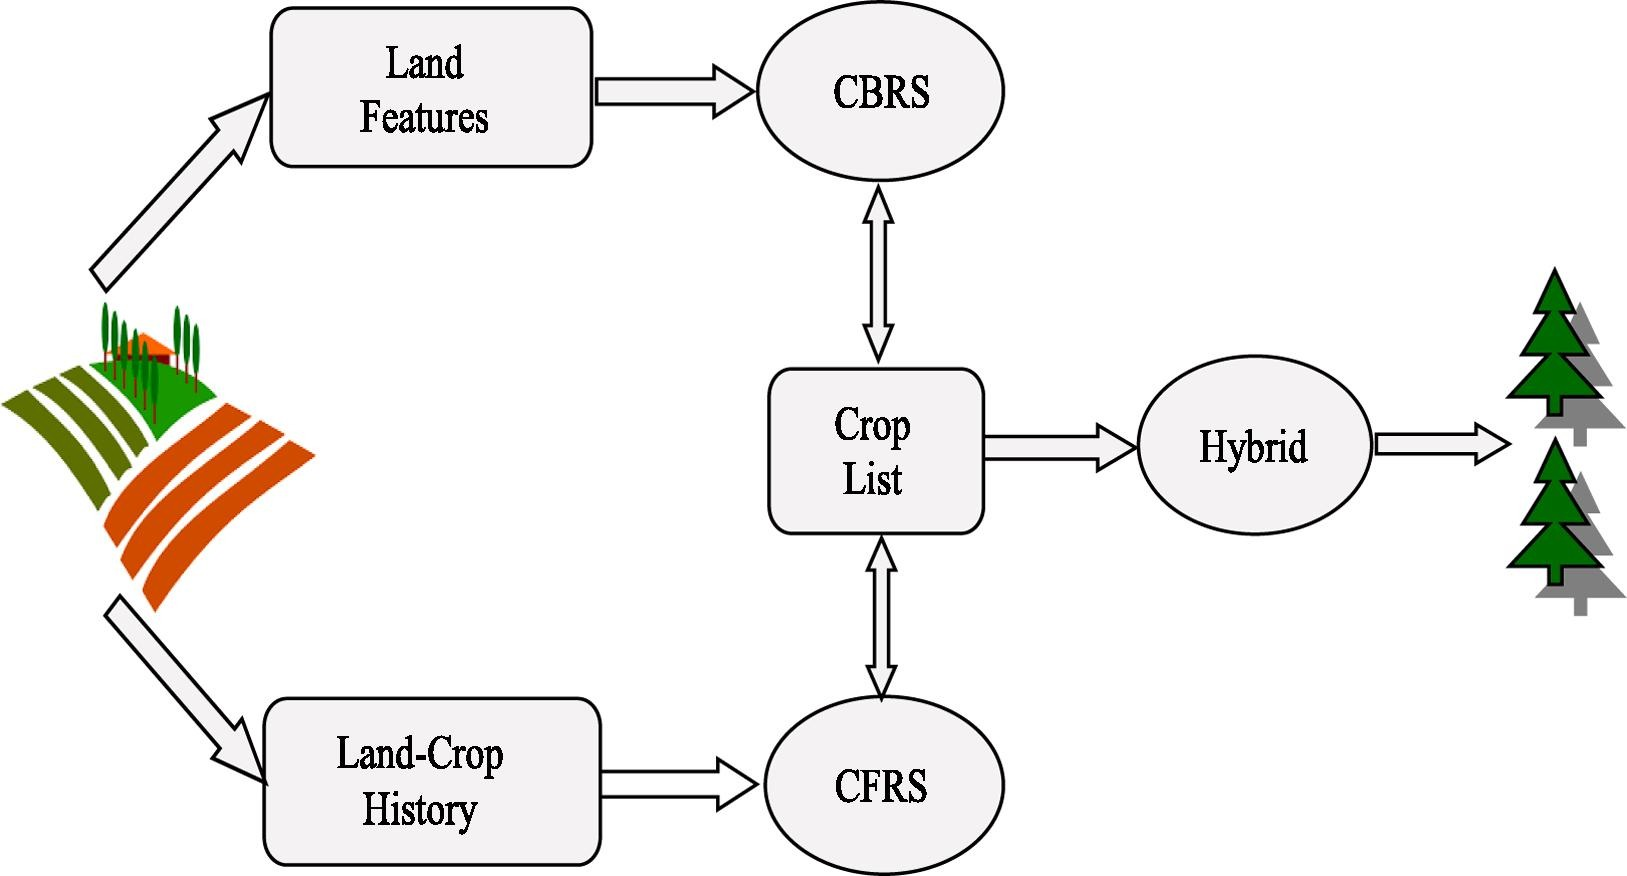
\includegraphics[width=\linewidth]{../graphics/Hybrid_RS_Land_Voorbeeld.jpg}
  \caption{Voorbeeld van hoe een hybride aanbevelingssysteem eruit kan zien \autocite{Patel2020}.} 
  \label{fig:hybrid_rs_land_voorbeeld}
\end{figure}

Het doel is een werkend proof-of-concept systeem te bouwen dat accurate en gepersonaliseerde aanbevelingen kan genereren, waarbij het vrijwel geen toegang heeft tot gevoelige gegevens van gebruikers. Door een combinatie van privacy behoudende technologieën, zoals FL en DP, vindt dit systeem een balans tussen bruikbaarheid en privacy. Als dit lukt, kan het een belangrijke stap zijn in de ontwikkeling van veilige en effectieve aanbevelingssystemen die vertrouwen winnen bij de gebruiker.

%---------- Stand van zaken ---------------------------------------------------
\section{Literatuurstudie}
\label{sec:literatuurstudie}

Aanbevelingssystemen zijn de laatste jaren enorm in opkomst en worden toegepast in verschillende sectoren. Ze zijn essentieel voor het bieden van gepersonaliseerde diensten aan gebruikers. Daarnaast vormen zulke diensten een effectieve inkomstenbron voor online bedrijven \autocite{Mazeh2020, Wang2018}. Echter, het gebruik van aanbevelingsdiensten vergt verzamelen van persoonlijke gegevens van gebruikers voor verwerking en analyse, wat gebruikers ongewenst vatbaar maakt voor privacyrisico's. Verder heeft elke serviceprovider een database met informatie over al zijn gebruikers \autocite{Wang2018, Lex2023, Yang2020, Friedman2015}.

Er zijn verschillende oplossingen uitgevonden om de privacy van gebruikers te beschermen. Eerste is Collaborative Filtering (CF), dit is een techniek die wordt gebruikt in aanbevelingssystemen om gebruikers te groeperen op basis van hun voorkeuren en interesses ten overzichte van andere gebruikers. Maar CF vereist een centrale server die de gegevens opslaat \autocite{Li2017,Wang2018}. Dit zorgt voor dat deze gebruikersgegevens kunnen worden misbruikt om privé informatie bekend te maken aan niet-vertrouwde partijen en om gebruikerskenmerken zoals geslacht of leeftijd af te leiden \autocite{Lex2023}. 
Differentional Privacy (DP) kan hierbij een oplossing bieden, uit \textcite{Friedman2015,Lex2023} volgt dat DP "is een rigoureus privacymodel dat ervoor zorgt dat de uitvoer van een berekening niet onthult of de gegevens van een specifieke persoon in de dataset zijn opgenomen". Dit wordt bereikt door zorgvuldig gekalibreerde ruis toe te voegen om de invloed van een enkele datapunt te maskeren.

Tweede techniek is Content Based (CB), aanbvelingssysteemen gebaseerd op CB bevelen items aan gebruikers aan op basis van de overeenkomsten tussen de inhoud van die items en voorkeuren van de gebruiker \autocite{Lops2010,Pazzani2007}. Hierbij worden verschillende datapunten van items en gebruikersprofielen geanalyseerd om patronen en voorkeuren te ontdekken en te groeperen. Hierin ligt ook het verschil met CF, waarbij de focus ligt op de overeenkomsten tussen gebruikers onderling. Nadelen van CB houden in: overspecialisatie, aanbevelingen hebben smal bereik van gebruikersinteresses, wat de ontdekking van nieuwe en diverse inhoud kan belemmeren en gedetailleerde analyse van gegevens, wat complex en tijdrovend kan zijn afhankelijk van de aard van de gegevens \autocite{Patel2020,Lops2010}.
In combinatie met Federated Learning (FL) kan CB verebterd worden. In plaats van gebruikersinformatie naar een centrale server te sturen, worden modellen getraind op het apparaat van de gebruikers zelf. Zo blijven persoonlijke gegevens lokaal bij de gebruiker en worden nooit uitgestuurd. Alleen geanonimiseerde modelupdates worden gedeeld met een centrale server, waardoor het systeem leert van de verzamelde inzichten zonder individuele gegevens te verzamelen \autocite{Wang2018, Lops2010}.

% Voor literatuurverwijzingen zijn er twee belangrijke commando's:
% \autocite{KEY} => (Auteur, jaartal) Gebruik dit als de naam van de auteur
%   geen onderdeel is van de zin.
% \textcite{KEY} => Auteur (jaartal)  Gebruik dit als de auteursnaam wel een
%   functie heeft in de zin (bv. ``Uit onderzoek door Doll & Hill (1954) bleek
%   ...'')

%---------- Methodologie ------------------------------------------------------
%// [ ] hoe wil ik DE en FL combineren 
%// [ ] tijdschatting gantt diagram opstellen, zie RM

\section{Methodologie}%
\label{sec:methodologie}

We passen het strtegie van verdeel en heers om dit probleem makkelijker op te lossen. Beschouw het hybride aanbevelingssysteem als een combinatie van twee subsystemen: een Content Based (CB) gebaseerde en Collaborative Filtering (CF) gebaseerde systeem. 

Hier beschrijf je hoe je van plan bent het onderzoek te voeren. Welke onderzoekstechniek ga je toepassen om elk van je onderzoeksvragen te beantwoorden? Gebruik je hiervoor literatuurstudie, interviews met belanghebbenden (bv.~voor requirements-analyse), experimenten, simulaties, vergelijkende studie, risico-analyse, PoC, \ldots?

Valt je onderwerp onder één van de typische soorten bachelorproeven die besproken zijn in de lessen Research Methods (bv.\ vergelijkende studie of risico-analyse)? Zorg er dan ook voor dat we duidelijk de verschillende stappen terug vinden die we verwachten in dit soort onderzoek!

Vermijd onderzoekstechnieken die geen objectieve, meetbare resultaten kunnen opleveren. Enquêtes, bijvoorbeeld, zijn voor een bachelorproef informatica meestal \textbf{niet geschikt}. De antwoorden zijn eerder meningen dan feiten en in de praktijk blijkt het ook bijzonder moeilijk om voldoende respondenten te vinden. Studenten die een enquête willen voeren, hebben meestal ook geen goede definitie van de populatie, waardoor ook niet kan aangetoond worden dat eventuele resultaten representatief zijn.

Uit dit onderdeel moet duidelijk naar voor komen dat je bachelorproef ook technisch voldoen\-de diepgang zal bevatten. Het zou niet kloppen als een bachelorproef informatica ook door bv.\ een student marketing zou kunnen uitgevoerd worden.

Je beschrijft ook al welke tools (hardware, software, diensten, \ldots) je denkt hiervoor te gebruiken of te ontwikkelen.

Probeer ook een tijdschatting te maken. Hoe lang zal je met elke fase van je onderzoek bezig zijn en wat zijn de concrete \emph{deliverables} in elke fase?

%---------- Verwachte resultaten ----------------------------------------------
\section{Verwacht resultaat, conclusie}%
\label{sec:verwachte_resultaten}

Hier beschrijf je welke resultaten je verwacht. Als je metingen en simulaties uitvoert, kan je hier al mock-ups maken van de grafieken samen met de verwachte conclusies. Benoem zeker al je assen en de onderdelen van de grafiek die je gaat gebruiken. Dit zorgt ervoor dat je concreet weet welk soort data je moet verzamelen en hoe je die moet meten.

Wat heeft de doelgroep van je onderzoek aan het resultaat? Op welke manier zorgt jouw bachelorproef voor een meerwaarde?

Hier beschrijf je wat je verwacht uit je onderzoek, met de motivatie waarom. Het is \textbf{niet} erg indien uit je onderzoek andere resultaten en conclusies vloeien dan dat je hier beschrijft: het is dan juist interessant om te onderzoeken waarom jouw hypothesen niet overeenkomen met de resultaten.



%%---------- Andere bijlagen --------------------------------------------------
% TODO: Voeg hier eventuele andere bijlagen toe. Bv. als je deze BP voor de
% tweede keer indient, een overzicht van de verbeteringen t.o.v. het origineel.
%\input{...}

%%---------- Backmatter, referentielijst ---------------------------------------

\backmatter{}

\setlength\bibitemsep{2pt} %% Add Some space between the bibliograpy entries
\printbibliography[heading=bibintoc]

\end{document}
